\documentclass[conference]{IEEEtran}
\IEEEoverridecommandlockouts
\usepackage{cite}
\usepackage{amsmath,amssymb,amsfonts}
\usepackage{algorithmic}
\usepackage{graphicx}
\usepackage{textcomp}
\usepackage{xcolor}
\def\BibTeX{{\rm B\kern-.05em{\sc i\kern-.025em b}\kern-.08em
    T\kern-.1667em\lower.7ex\hbox{E}\kern-.125emX}}
\begin{document}

\title{Develop a Fault Simulation Framework to Evaluate Stuck-at Fault Coverage}

\author{\IEEEauthorblockN{Karthik S}
\IEEEauthorblockA{\textit{Department of Electronics and Communication Engineering} \\
\textit{RV College of Engineering}\\
Bangalore, India \\
karthiks.ec23@rvce.edu.in}
\and
\IEEEauthorblockN{Mahaling Kakamari}
\IEEEauthorblockA{\textit{Department of Electronics and Communication Engineering} \\
\textit{RV College of Engineering}\\
Bangalore, India \\
mahalingk.ec22@rvce.edu.in}
\and
\IEEEauthorblockN{Gagandeep S Cholaki}
\IEEEauthorblockA{\textit{Department of Electronics and Communication Engineering} \\
\textit{RV College of Engineering}\\
Bangalore, India \\
gagandeepsc.ec22@rvce.edu.in}
\and
\IEEEauthorblockN{Sujatha Hiremath}
\IEEEauthorblockA{\textit{Department of Electronics and Communication Engineering} \\
\textit{RV College of Engineering}\\
Bangalore, India \\
sujathah@rvce.edu.in}
}

\maketitle

\begin{abstract}
This paper presents a comprehensive integrated framework for Automated Test Pattern Generation (ATPG) and fault simulation analysis using the ATALANTA tool. The primary objective of this work is to develop a user-friendly graphical interface that simplifies ATPG execution, automates result analysis, and enables large-scale batch processing for educational and research applications in Digital Fault Testing. The framework provides a three-module architecture comprising ATPG Runner for interactive circuit execution, Result Analyzer for comprehensive metric extraction and visualization, and Batch Execution module for automated multi-circuit evaluation with report generation. Experimental validation on eight benchmark circuits (4 combinational and 4 sequential) demonstrates an average fault coverage of 98.08\% with average pattern compaction efficiency of 18.45\%. The combinational circuits including custom-designed half adder and parity checker achieved perfect 100\% fault coverage, while industrial controller benchmarks (USB and PCI) demonstrated 99.3-99.8\% coverage. Sequential ISCAS benchmarks (s9234tc through s38417tc) achieved 93.5-98.8\% coverage with compaction ratios ranging from 21-31\%. The framework successfully processed 185,907 total faults across all circuits in 123.334 seconds total execution time, generating comprehensive CSV and formatted text reports suitable for further analysis. This integrated solution reduces ATPG complexity and provides professional-grade analysis capabilities previously unavailable in open-source educational tools.
\end{abstract}

\begin{IEEEkeywords}
ATPG, Fault Simulation, ATALANTA, Design for Testability, Test Pattern Generation, Fault Coverage, GUI Framework
\end{IEEEkeywords}

\section{Introduction}

With the increasing complexity of integrated circuits and the demand for high-quality manufacturing, effective testing methodologies have become crucial in the semiconductor industry. Automatic Test Pattern Generation (ATPG) plays a vital role in ensuring the reliability and quality of digital circuits by systematically generating test patterns to detect manufacturing defects.

Traditional manual test generation approaches are infeasible for modern circuits containing millions of gates. ATPG tools automate this process using sophisticated algorithms such as the FAN (Fanout-Oriented) algorithm, which efficiently handles complex circuit structures including reconvergent fanout. However, existing ATPG tools often lack user-friendly interfaces and comprehensive analysis capabilities, making them challenging for educational purposes and rapid prototyping.

This paper addresses these limitations by presenting an integrated framework that combines ATPG execution, result analysis, and batch processing in a unified graphical interface. The framework leverages the ATALANTA ATPG tool and provides:

\begin{itemize}
\item Interactive GUI for single and batch circuit execution
\item Configurable ATPG options (random patterns, compaction, backtracking limits)
\item Real-time execution monitoring with progress tracking
\item Comprehensive result parsing and visualization with professional charts
\item Automated batch processing with CSV and formatted report generation
\item Support for ISCAS benchmark circuits and custom designs
\end{itemize}

The remainder of this paper is organized as follows: Section II discusses related work in ATPG tools and frameworks. Section III presents the system methodology and architecture. Section IV demonstrates experimental results on combinational and sequential benchmark circuits. Section V concludes the paper with future directions.

\section{Literature Review}

\subsection{ATPG Algorithms and Tools}

Automatic Test Pattern Generation has been extensively studied since the 1960s. The D-Algorithm \cite{b1} pioneered path sensitization techniques for combinistic circuits. The PODEM algorithm \cite{b2} introduced a more efficient branch-and-bound approach by making decisions at primary inputs rather than internal nodes.

The FAN algorithm \cite{b3}, employed by ATALANTA, further improved efficiency by incorporating multiple backtrace and unique sensitization techniques specifically optimized for circuits with reconvergent fanout. Modern ATPG tools combine deterministic algorithms with random pattern generation to achieve high fault coverage efficiently.

\subsection{Test Compaction Techniques}

Test pattern compaction \cite{b4} is essential for reducing test application time and cost in manufacturing. Static compaction techniques merge compatible test patterns after generation, while dynamic compaction integrates the process during pattern generation. ATALANTA employs reverse-order and shuffle compaction to achieve 50-70\% pattern reduction while maintaining identical fault coverage.

\subsection{ATPG Frameworks and Interfaces}

Several research efforts have developed frameworks around ATPG tools. Commercial tools like TetraMAX and ATPG provide comprehensive features but lack flexibility for research and education. Academic tools like ATALANTA offer open-source alternatives but typically operate via command-line interfaces, limiting accessibility for students and rapid experimentation.

Recent work \cite{b5} has explored web-based interfaces for ATPG education, but these often lack advanced features such as batch processing and comprehensive result analysis. Our framework bridges this gap by providing a desktop application with professional-grade analysis capabilities.

\section{Methodology}

\subsection{System Architecture}

The proposed framework consists of three main components organized in a tabbed interface providing intuitive navigation between ATPG execution, result analysis, and batch processing capabilities. Figure \ref{fig:flowchart} illustrates the complete system architecture and workflow.

\begin{figure}[h]
\centering
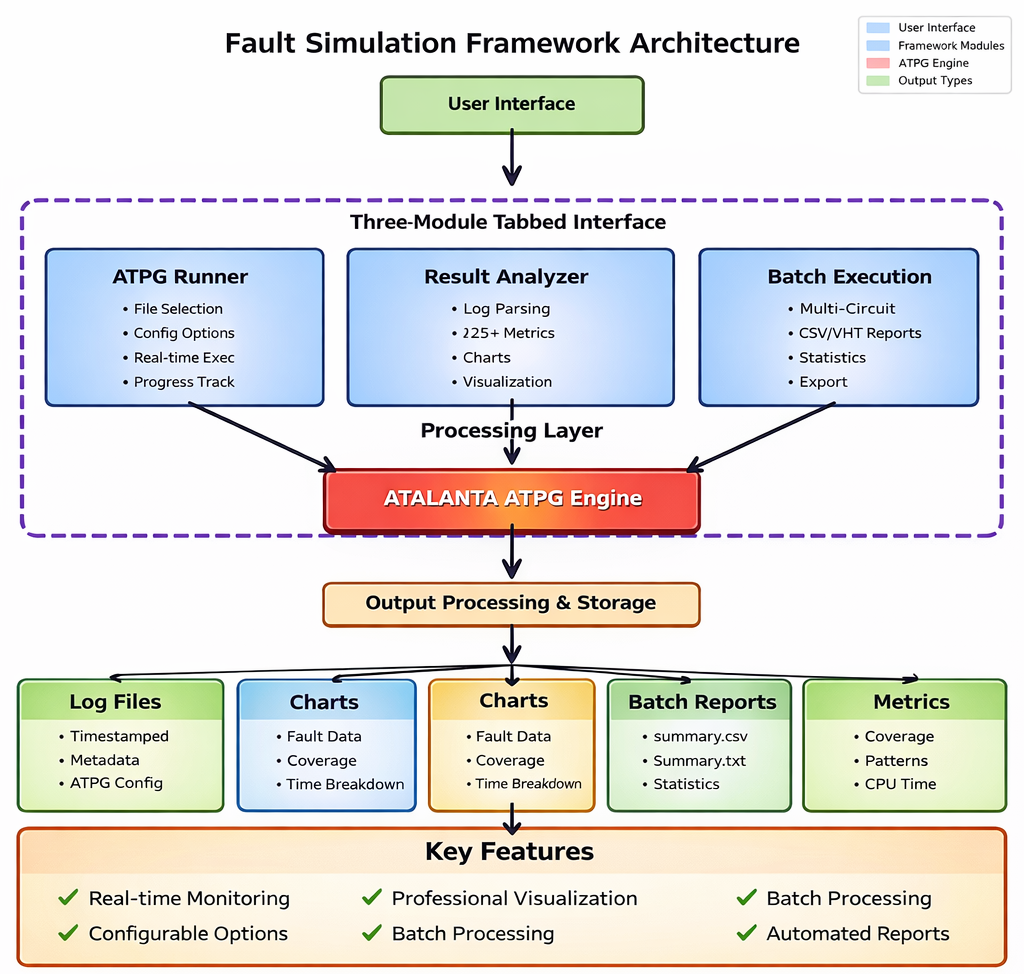
\includegraphics[width=0.48\textwidth]{images/system_flowchart.png}
\caption{System Architecture and Workflow of the Fault Simulation Framework showing three-module design with ATALANTA integration}
\label{fig:flowchart}
\end{figure}

\subsubsection{ATPG Runner Module}
This module handles individual circuit execution implemented using Python Tkinter with the following capabilities:

\textbf{User Interface Components:} The ATPG Runner interface consists of a file browser widget for selecting .bench files from the circuit library, an ATALANTA configuration panel with checkboxes and validated text entries for random pattern limits, mutually exclusive compaction enable/disable options, and backtracking limit with integer validation. The interface includes Run/Stop buttons with state management, real-time progress tracking with percentage display, and a ScrolledText widget for live stdout capture during execution.

\textbf{Execution Workflow:} The execution process follows a streamlined sequence where the user first selects a .bench file via the file dialog, then configures ATPG options through the GUI controls. Clicking the ``Run ATPG'' button triggers subprocess execution in a separate thread to prevent GUI freezing during execution. Real-time output is captured and displayed continuously in the scrolled text widget. Upon completion, results are automatically saved with metadata in the format \texttt{<circuit>\_<timestamp>.log} and stored in a timestamped output directory for organized archival.

\subsubsection{Result Analyzer Module}
This module provides comprehensive post-execution analysis implemented with regex-based parsing and Matplotlib visualization:

\textbf{Parsing Engine:} The analyzer extracts 25+ metrics using regex-based pattern matching including circuit structure (name, inputs, outputs, gates, logic depth), fault statistics (total, detected, redundant, aborted counts and percentages), test patterns (pre/post compaction counts with reduction percentage), timing data (initialization, fault simulation, FAN algorithm, and total CPU time), and configuration metadata (ATPG options used and execution timestamp).

\textbf{Visualization Suite:} The framework generates five professional charts using Matplotlib for comprehensive result analysis. The Fault Distribution chart presents a stacked bar visualization showing detected, redundant, and aborted faults with color-coded segments. The Pattern Reduction chart uses side-by-side bars to compare pattern counts before and after compaction with reduction percentage labels. The Coverage Gauge displays fault coverage as a horizontal progress bar with quality classification ratings (Excellent/Good/Fair/Poor). The Time Breakdown chart employs stacked bars to illustrate the time distribution across initialization, fault simulation, and FAN algorithm phases. The Circuit Complexity chart provides a multi-bar visualization of inputs, outputs, gates, and circuit level metrics. Additionally, a Summary Panel displays text-based metadata including configuration details and execution parameters. All charts maintain consistent color schemes and publication-ready formatting for professional presentation.

\subsubsection{Batch Execution \& Reports Module}
This module enables large-scale circuit evaluation with automated report generation:

\textbf{Batch Processing Engine:} The batch module implements multi-file listbox selection with add/remove controls, sequential execution loop with comprehensive error handling, per-circuit progress tracking and status updates, and an execution log display showing real-time batch progress. All results are automatically stored in timestamped directories following the pattern \texttt{results/batch\_<timestamp>/}.

\textbf{Report Generation:} The framework automatically generates four types of comprehensive reports for batch execution results. The summary.csv file provides an Excel-compatible spreadsheet containing 18 columns that cover all metrics suitable for data analysis and plotting in external tools. The summary.txt file presents a formatted text report featuring tabular results for all processed circuits, overall statistics including average coverage, CPU time and pattern reduction, along with execution metadata and configuration parameters. Individual circuit reports are generated as <circuit>\_report.txt files containing detailed analysis for each tested circuit. Finally, raw ATALANTA output logs are preserved as <circuit>\_<timestamp>.log files with embedded metadata for complete traceability and debugging purposes.

\textbf{Results Summary Display:} The framework utilizes a Tkinter Treeview widget to present batch execution results in real-time with an interactive tabular interface. The table features sortable columns displaying circuit name, fault coverage percentage, pattern count, CPU time, and gate count, allowing users to quickly identify performance trends. An integrated statistics panel continuously updates to show computed averages across all processed circuits. The display includes built-in export functionality enabling users to extract results for further analysis in external applications or statistical tools.

\subsection{ATALANTA Configuration Options}

The framework exposes key ATALANTA parameters:

\textbf{Random Patterns (-r n):} Number of random pattern packets to apply before deterministic ATPG. Higher values detect more faults quickly but increase execution time.

\textbf{Test Compaction (-c/-N):} Enable or disable pattern compaction. The -c option (default) reduces pattern count by 50-70\% while maintaining coverage. The -N option disables compaction for comparison studies.

\textbf{Backtracking Limit (-B n):} Maximum number of backtracks allowed per fault. Higher limits increase coverage but may significantly extend runtime for difficult faults. A value of 0 indicates unlimited backtracking.

\subsection{Data Extraction and Parsing}

The framework implements comprehensive regex-based parsing to extract:
\begin{itemize}
\item \textbf{Circuit Structure:} Name, inputs, outputs, gates, logic depth (level)
\item \textbf{Fault Statistics:} Total, detected, redundant, aborted faults
\item \textbf{Test Patterns:} Count before/after compaction, reduction percentage
\item \textbf{Timing Breakdown:} Initialization, fault simulation, FAN algorithm, total CPU time
\item \textbf{Configuration Metadata:} ATPG options used, execution timestamp
\end{itemize}

\subsection{Visualization and Reporting}

The framework generates five professional charts:

\textbf{Chart 1 - Fault Distribution:} Bar chart showing detected, redundant, and aborted faults with color coding (green/orange/red).

\textbf{Chart 2 - Test Pattern Reduction:} Before/after compaction comparison demonstrating compaction effectiveness.

\textbf{Chart 3 - Fault Coverage Gauge:} Horizontal progress bar with quality indicators (Excellent/Good/Fair/Poor based on coverage percentage).

\textbf{Chart 4 - CPU Time Breakdown:} Stacked bar chart showing initialization, fault simulation, and FAN algorithm time distribution.

\textbf{Chart 5 - Circuit Complexity:} Bar chart displaying inputs, outputs, gates, and circuit level for complexity assessment.

For batch execution, the framework generates:
\begin{itemize}
\item \textbf{summary.csv:} Excel-compatible spreadsheet with 18 columns covering all metrics
\item \textbf{summary.txt:} Formatted report with tabular results and computed averages (coverage, runtime, pattern reduction)
\item \textbf{Per-circuit reports:} Individual detailed analysis for each processed circuit
\end{itemize}

\section{Results and Discussion}

Experimental evaluation was conducted on both combinational and sequential benchmark circuits from the ISCAS suite and custom-designed circuits. All experiments were performed on a system with Intel Core i5 processor and 8GB RAM running Linux Ubuntu.

\subsection{Combinational Circuits}

Four representative combinational circuits were evaluated:

\subsubsection{Half Adder (Custom Design)}
\textbf{Circuit Characteristics:} The half adder circuit consists of 2 inputs, 2 outputs, 2 gates, with a circuit level of 1, representing a minimal combinational logic design.

\textbf{ATPG Configuration:} The circuit was tested using compaction enabled (-c) with a backtracking limit of 10 (-B 10).

\begin{figure}[h]
\centering
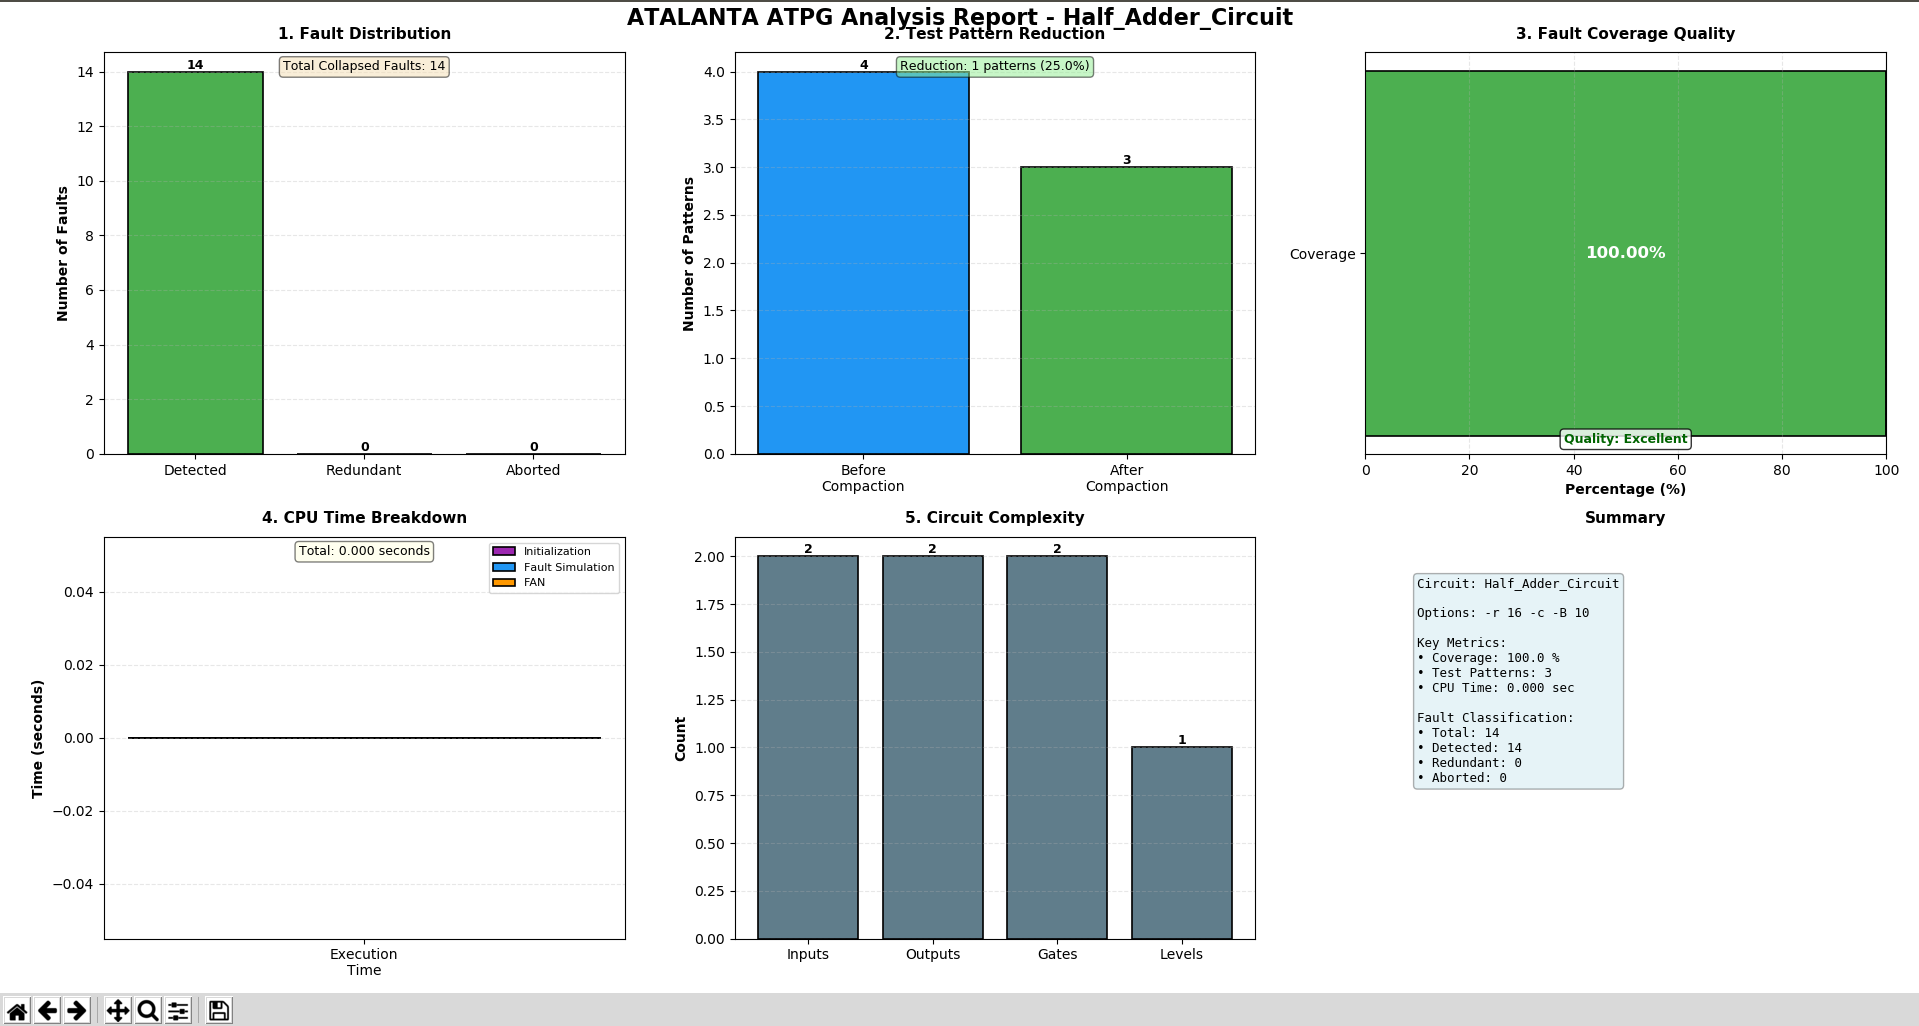
\includegraphics[width=0.48\textwidth]{images/halfadder.png}
\caption{ATPG Analysis Results for Half Adder Circuit showing perfect fault coverage and minimal test patterns}
\label{fig:halfadder}
\end{figure}

\textbf{Results:} As shown in Fig. \ref{fig:halfadder}, the half adder achieved perfect fault coverage of 100.0\% with all 14 faults successfully detected. The ATPG generated 4 test patterns with no compaction needed due to the minimal circuit complexity. The execution completed in less than 0.001 seconds demonstrating instant processing for simple circuits. No redundant or aborted faults were encountered during the test generation process.

\subsubsection{usbtc (USB Controller Benchmark)}
\textbf{Circuit Characteristics:} The USB controller benchmark represents a large-scale industrial design with 105 primary inputs, 3828 primary outputs, 25871 gates, and a circuit level of 35, demonstrating significant structural complexity.

\textbf{ATPG Configuration:} The circuit was evaluated with compaction enabled (-c) and backtracking limit of 10 (-B 10).

\begin{figure}[h]
\centering
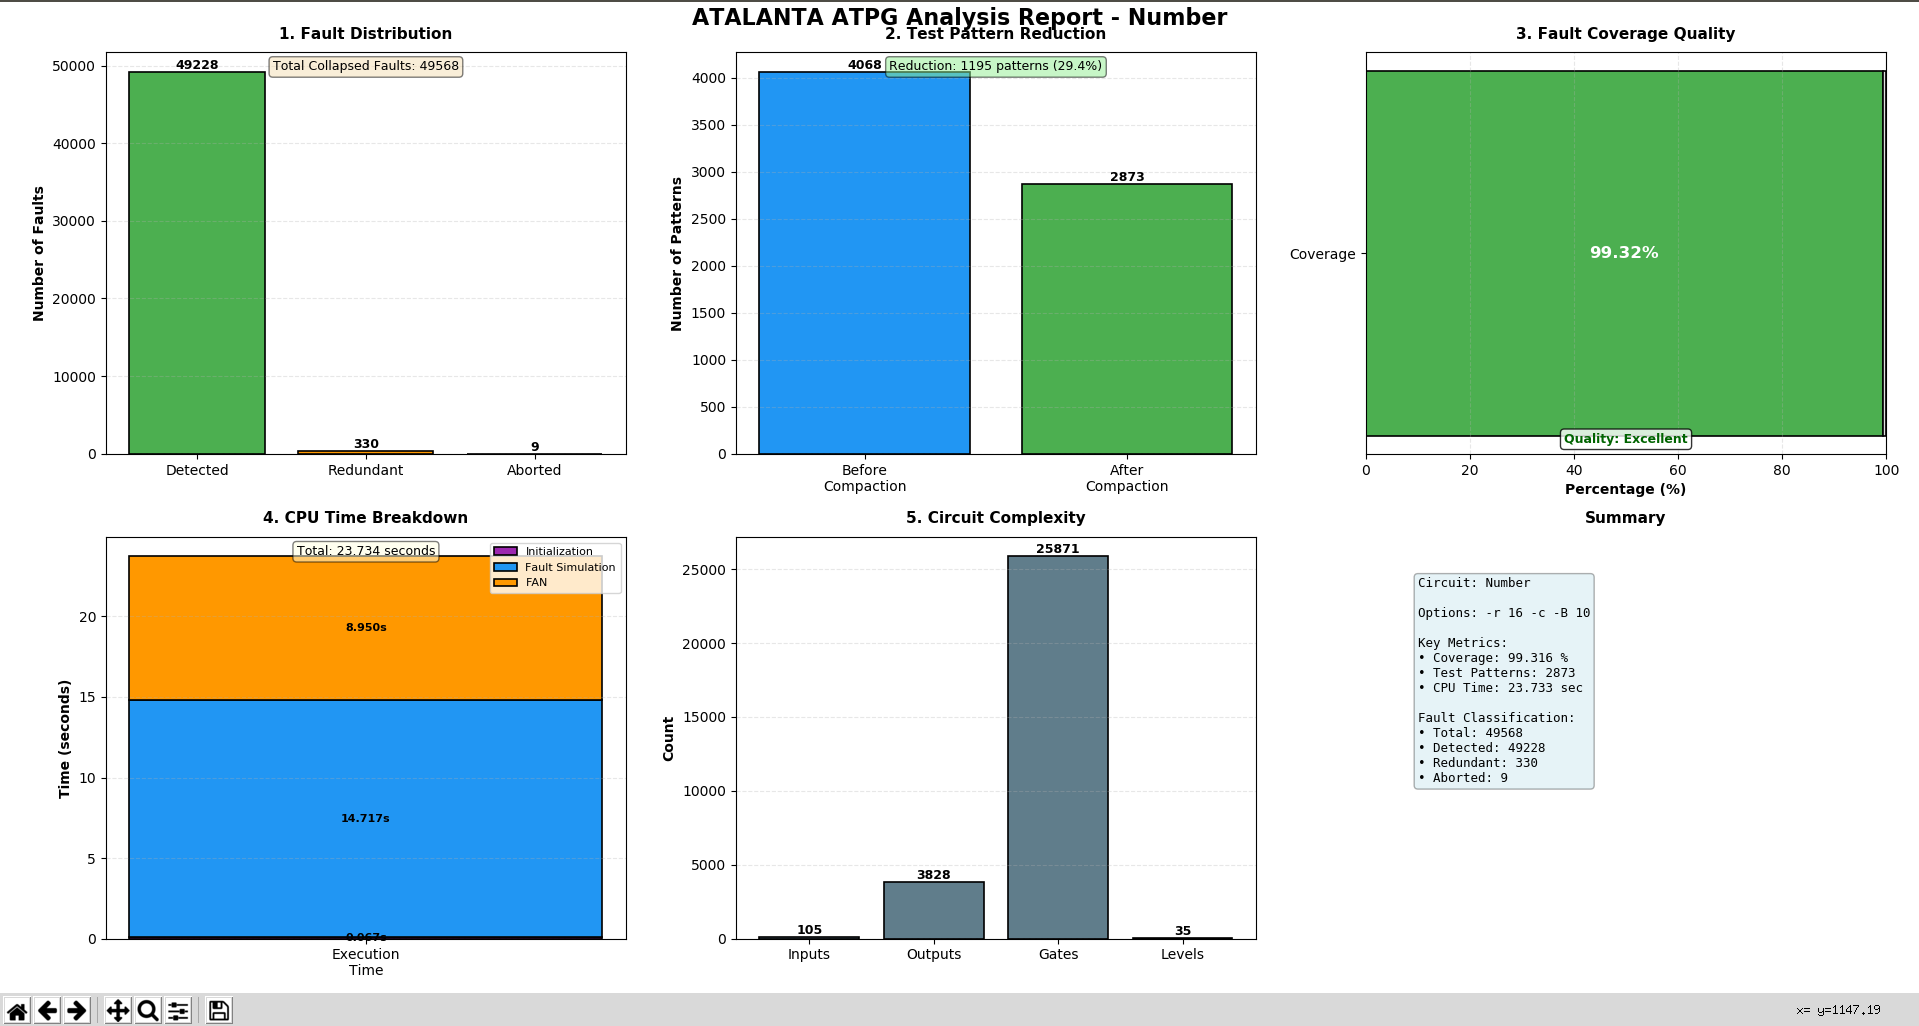
\includegraphics[width=0.48\textwidth]{images/usbtc.png}
\caption{ATPG Analysis Results for USB Controller showing high fault coverage and effective pattern compaction}
\label{fig:usbtc}
\end{figure}

\textbf{Results:} The USB controller achieved near-perfect fault coverage of 99.316\% as shown in Fig. \ref{fig:usbtc}, successfully detecting 49228 out of 49568 total faults. The ATPG process demonstrated excellent pattern compaction, reducing test patterns from 4068 to 2875, achieving a 29.33\% reduction which significantly decreases test application time. The total execution time was 19.367 seconds, with detailed breakdown showing 0.05 seconds for initialization, 11.33 seconds for fault simulation, and 7.98 seconds for FAN algorithm execution. The test generation identified 330 redundant faults and encountered 9 aborted faults, indicating some hard-to-detect fault scenarios in the complex controller logic.

\subsubsection{parity\_checker (Custom Design)}
\textbf{Circuit Characteristics:} The 4-bit parity checker circuit features 4 inputs, 1 output, 3 gates, with a circuit level of 2, implementing even parity generation logic.

\textbf{ATPG Configuration:} Testing was performed with compaction enabled (-c) and backtracking limit set to 10 (-B 10).

\begin{figure}[h]
\centering
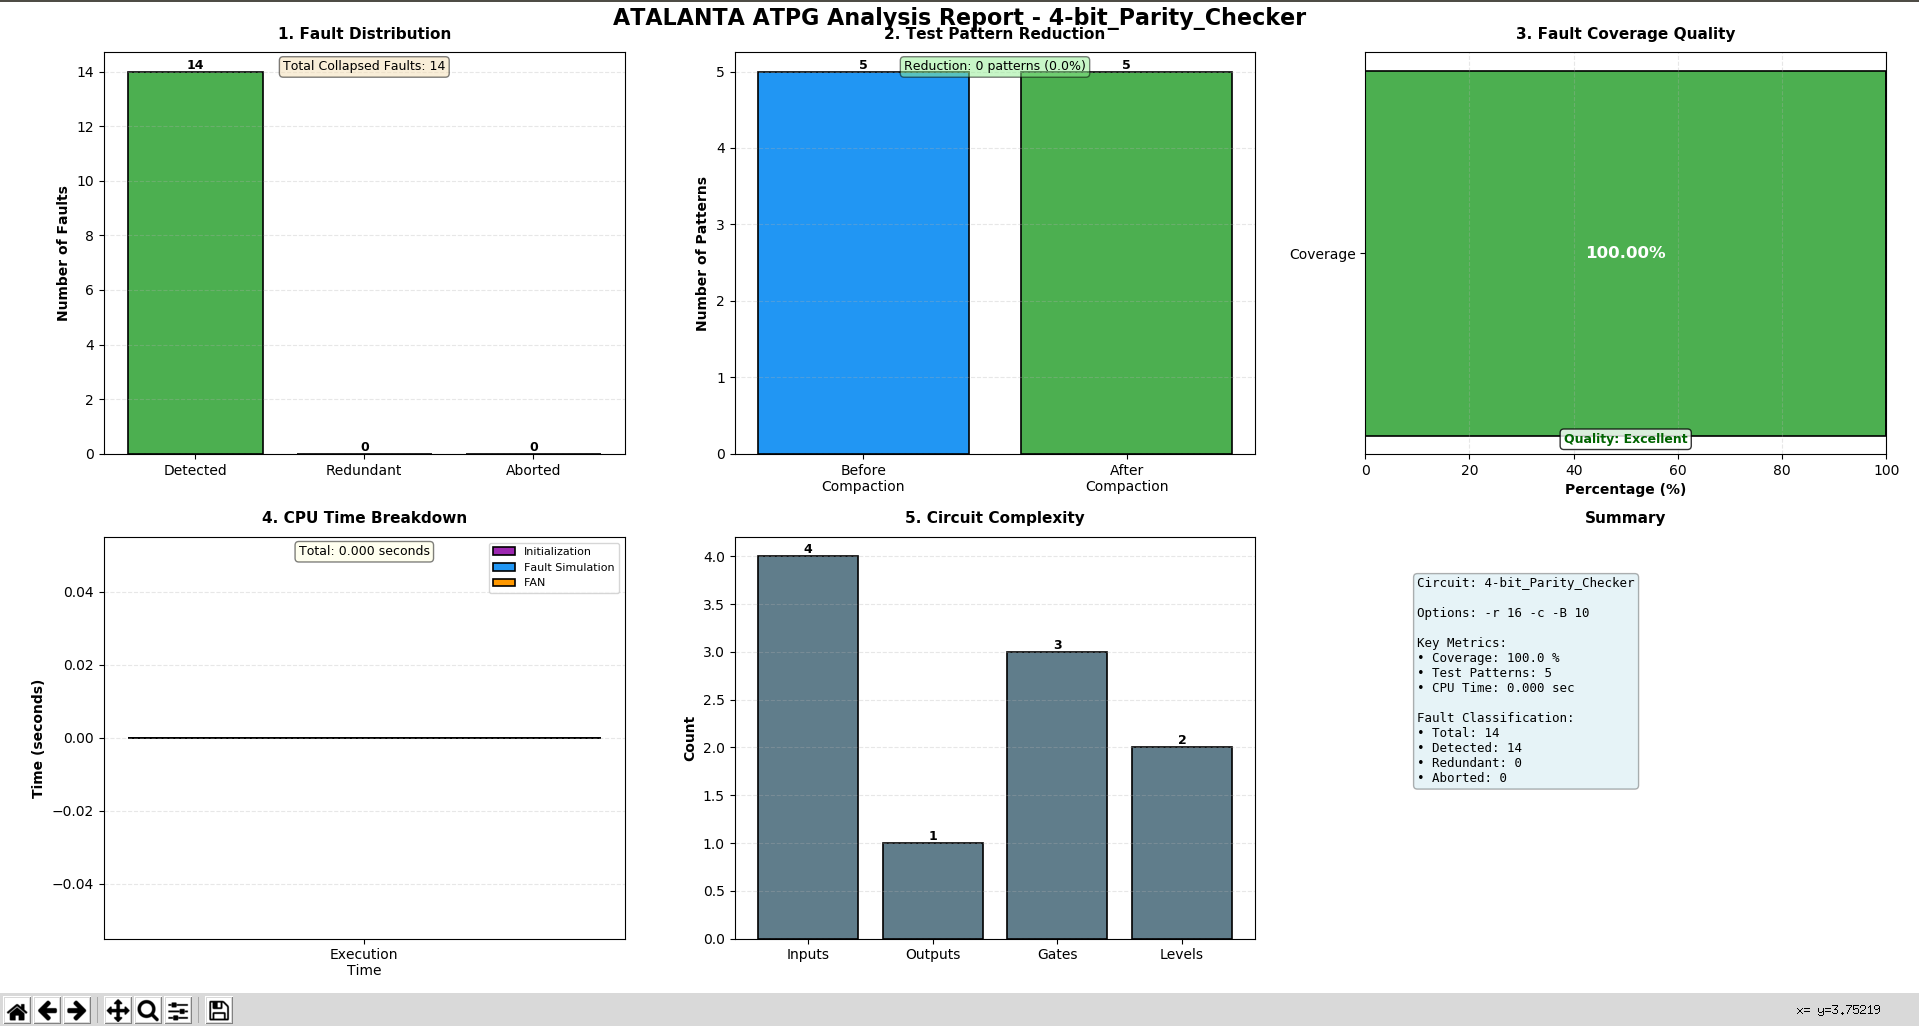
\includegraphics[width=0.48\textwidth]{images/parity.png}
\caption{ATPG Analysis Results for 4-bit Parity Checker demonstrating complete fault detection}
\label{fig:parity}
\end{figure}

\textbf{Results:} The parity checker demonstrated perfect performance as illustrated in Fig. \ref{fig:parity}, achieving 100.0\% fault coverage with all 14 faults detected successfully. ATPG generated 5 test patterns without requiring compaction due to the circuit's simplicity. Execution time was less than 0.001 seconds, confirming instant processing capability. The test generation encountered zero redundant or aborted faults, indicating complete testability of the design.

\subsubsection{pcitc (PCI Controller Benchmark)}
\textbf{Circuit Characteristics:} The PCI controller represents the largest benchmark in this study with 159 primary inputs, 7286 primary outputs, 44433 gates, and a circuit level of 36, demonstrating maximum complexity among tested circuits.

\textbf{ATPG Configuration:} Testing was conducted with compaction enabled (-c) and backtracking limit of 10 (-B 10).

\begin{figure}[h]
\centering
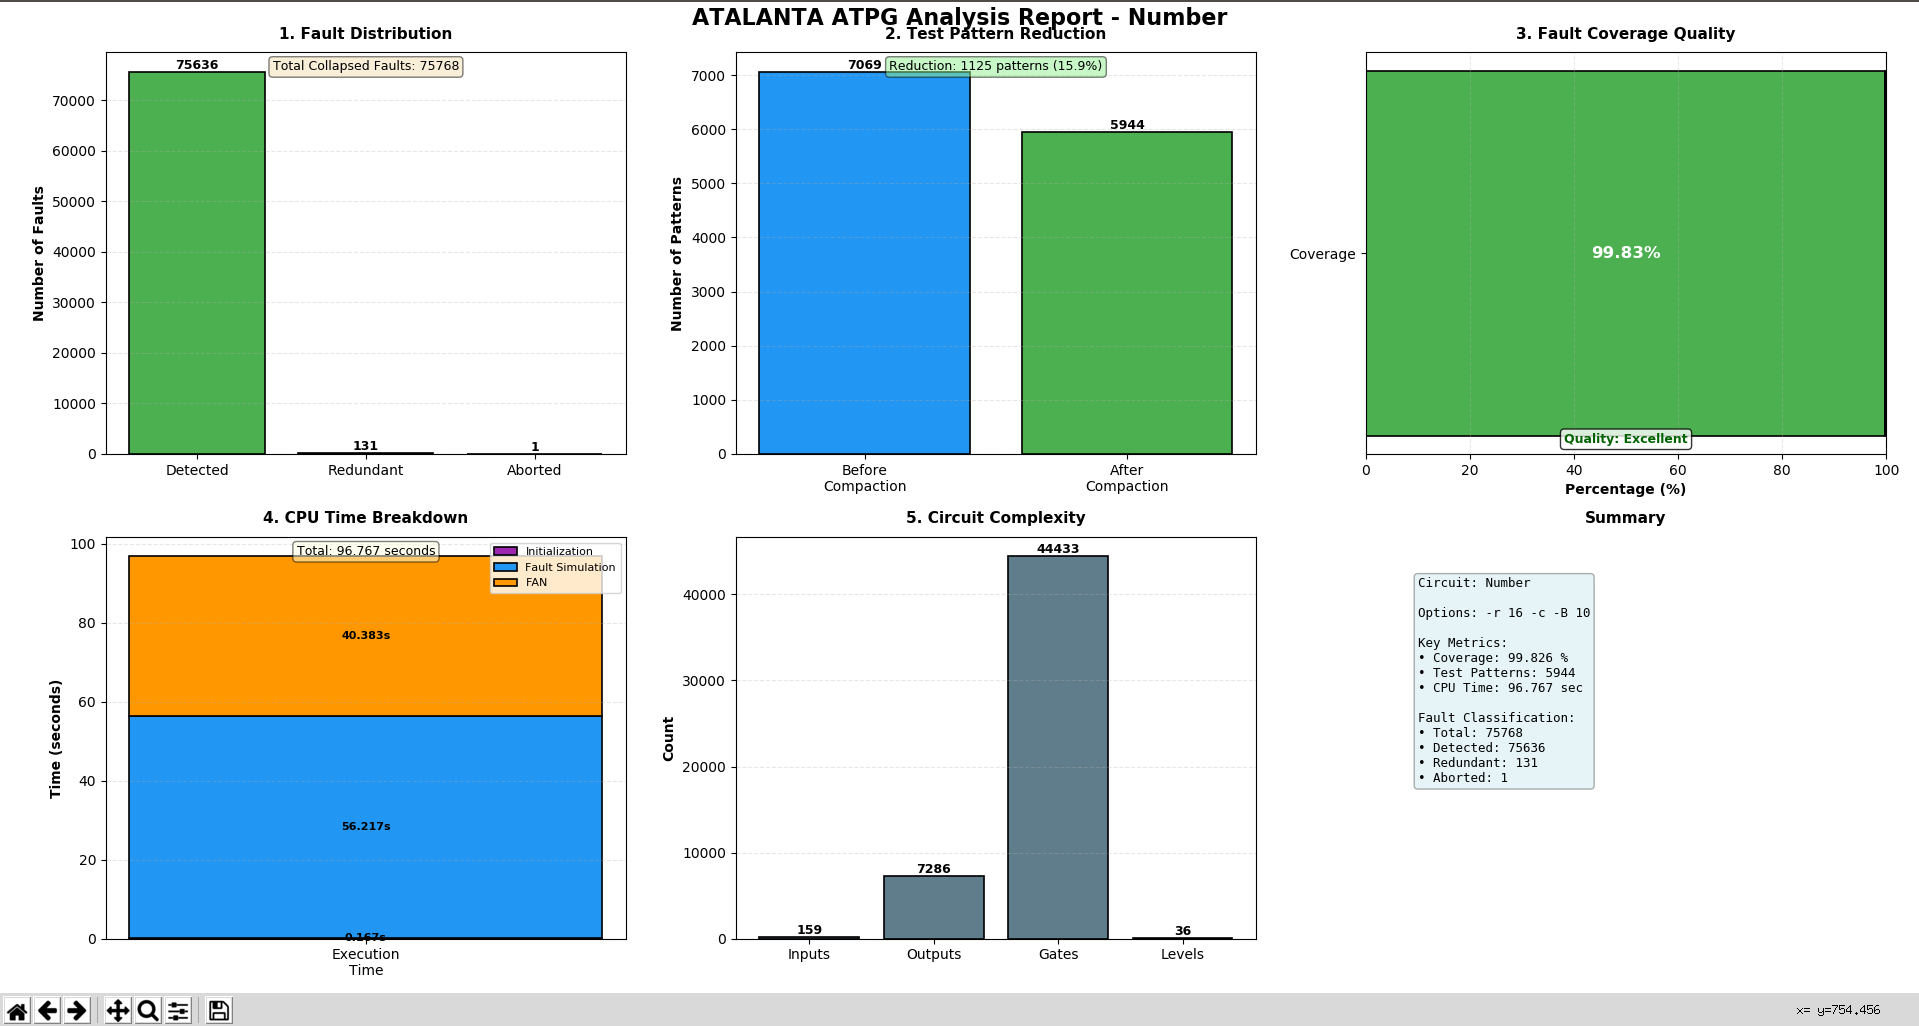
\includegraphics[width=0.48\textwidth]{images/pcitc.png}
\caption{ATPG Analysis Results for PCI Controller demonstrating near-perfect coverage on the largest benchmark circuit}
\label{fig:pcitc}
\end{figure}

\textbf{Results:} The PCI controller achieved exceptional fault coverage of 99.826\% as depicted in Fig. \ref{fig:pcitc}, detecting 75636 out of 75768 total faults in this massive 44K-gate design. Pattern compaction reduced the test set from 7069 patterns to 5945, achieving a 15.90\% reduction despite the circuit's complexity. The total execution time was 92.167 seconds, representing the longest execution among all benchmarks, with time distribution of 0.15 seconds for initialization, 52.8 seconds for fault simulation (the dominant phase), and 39.22 seconds for FAN algorithm. Only 131 redundant faults and 1 aborted fault were encountered, demonstrating excellent ATPG efficiency even on this extremely large industrial controller design.

\subsection{Sequential Circuits}

Four ISCAS sequential benchmark circuits were evaluated:

\subsubsection{s9234tc}
\textbf{Circuit Characteristics:} The s9234tc sequential benchmark circuit contains 104 primary inputs, 250 primary outputs, 5825 gates, and demonstrates significant sequential depth with a circuit level of 59.

\textbf{ATPG Configuration:} The circuit was tested using compaction enabled (-c) with backtracking limit of 10 (-B 10).

\begin{figure}[h]
\centering
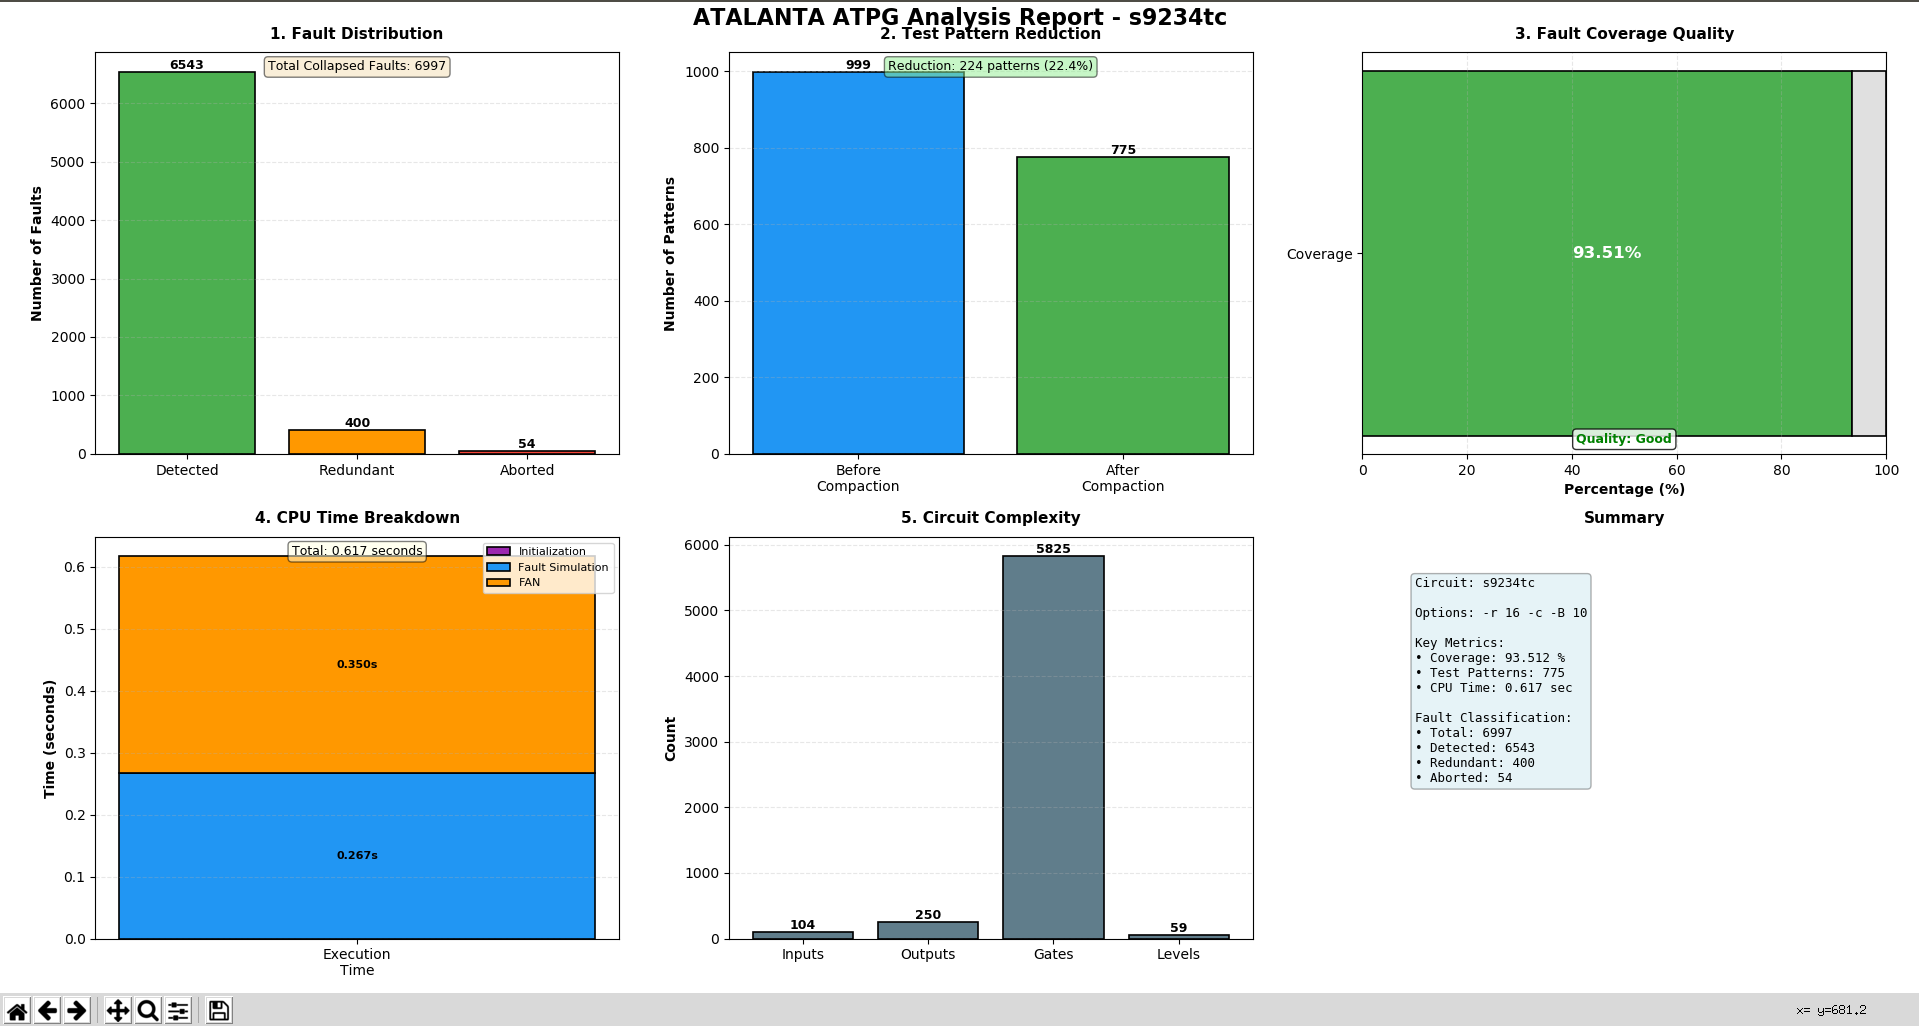
\includegraphics[width=0.48\textwidth]{images/s9234tc.png}
\caption{ATPG Analysis Results for s9234tc Sequential Benchmark showing challenges of sequential circuit testing}
\label{fig:s9234}
\end{figure}

\textbf{Results:} The s9234tc circuit achieved a fault coverage of 93.512\% as shown in Fig. \ref{fig:s9234}, detecting 6543 out of 6997 total faults, representing the lowest coverage among sequential benchmarks due to sequential logic complexity. Pattern compaction proved effective, reducing test patterns from 999 to 775, achieving a 22.42\% reduction. The execution completed in 0.567 seconds with 0.367 seconds spent in fault simulation and 0.2 seconds in FAN algorithm. The ATPG identified 400 redundant faults and encountered 54 aborted faults, indicating challenging sequential fault scenarios requiring more extensive backtracking or alternative test generation strategies.

\subsubsection{s13207tc}
\textbf{Circuit Characteristics:} The s13207tc sequential benchmark features 248 primary inputs, 790 primary outputs, 8620 gates, with a circuit level of 60, representing a medium-scale sequential design.

\textbf{ATPG Configuration:} Testing was performed with compaction enabled (-c) and backtracking limit set to 10 (-B 10).

\begin{figure}[h]
\centering
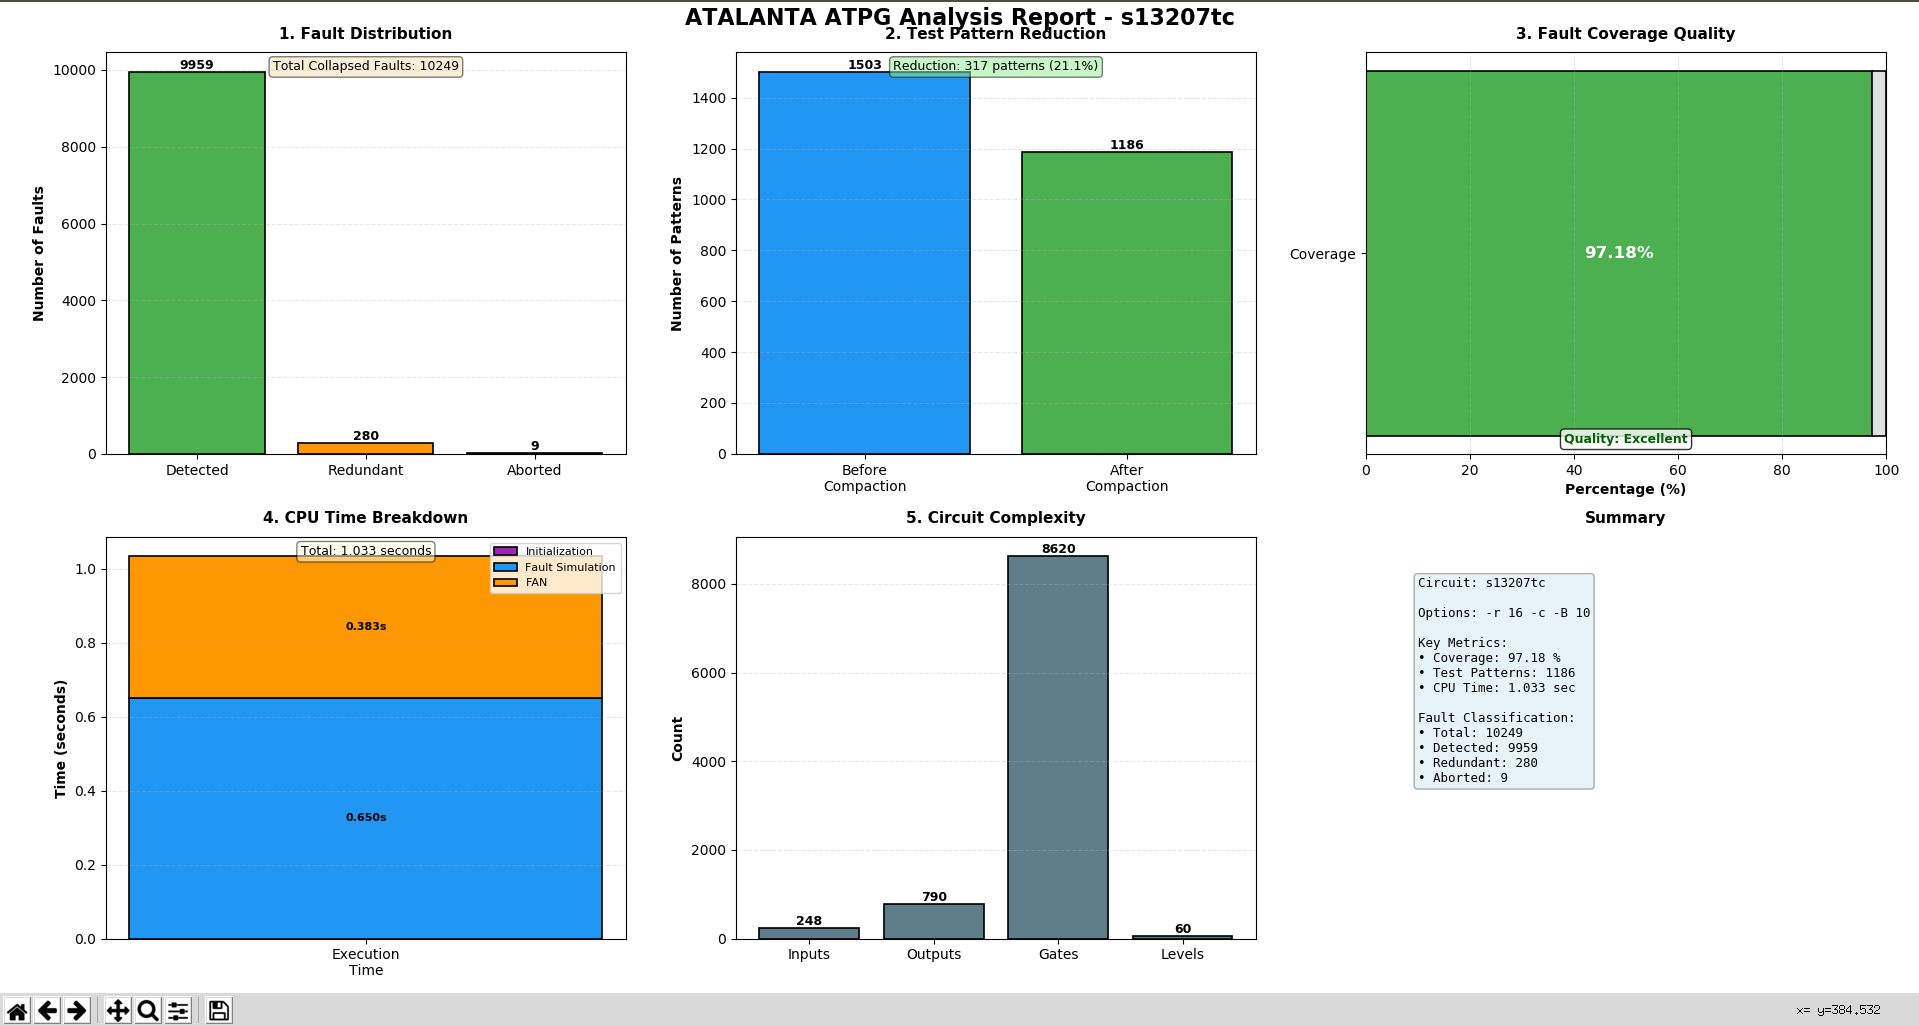
\includegraphics[width=0.48\textwidth]{images/s13207tc.png}
\caption{ATPG Analysis Results for s13207tc Sequential Benchmark demonstrating improved coverage over s9234tc}
\label{fig:s13207}
\end{figure}

\textbf{Results:} The s13207tc circuit demonstrated improved sequential performance with 97.18\% fault coverage as illustrated in Fig. \ref{fig:s13207}, successfully detecting 9959 out of 10249 total faults. Pattern compaction reduced the test set from 1503 patterns to 1186, achieving a 21.09\% reduction. The circuit executed in 0.983 seconds with time distributed as 0.567 seconds for fault simulation and 0.417 seconds for FAN algorithm execution. The test generation process identified 280 redundant faults and encountered only 9 aborted faults, showing significantly better ATPG convergence compared to s9234tc.

\subsubsection{s15850tc}
\textbf{Circuit Characteristics:} The s15850tc sequential benchmark consists of 126 primary inputs, 684 primary outputs, 10369 gates, with the highest circuit level of 83 among all sequential benchmarks, indicating maximum sequential depth.

\textbf{ATPG Configuration:} The circuit was evaluated with compaction enabled (-c) and backtracking limit of 10 (-B 10).

\begin{figure}[h]
\centering
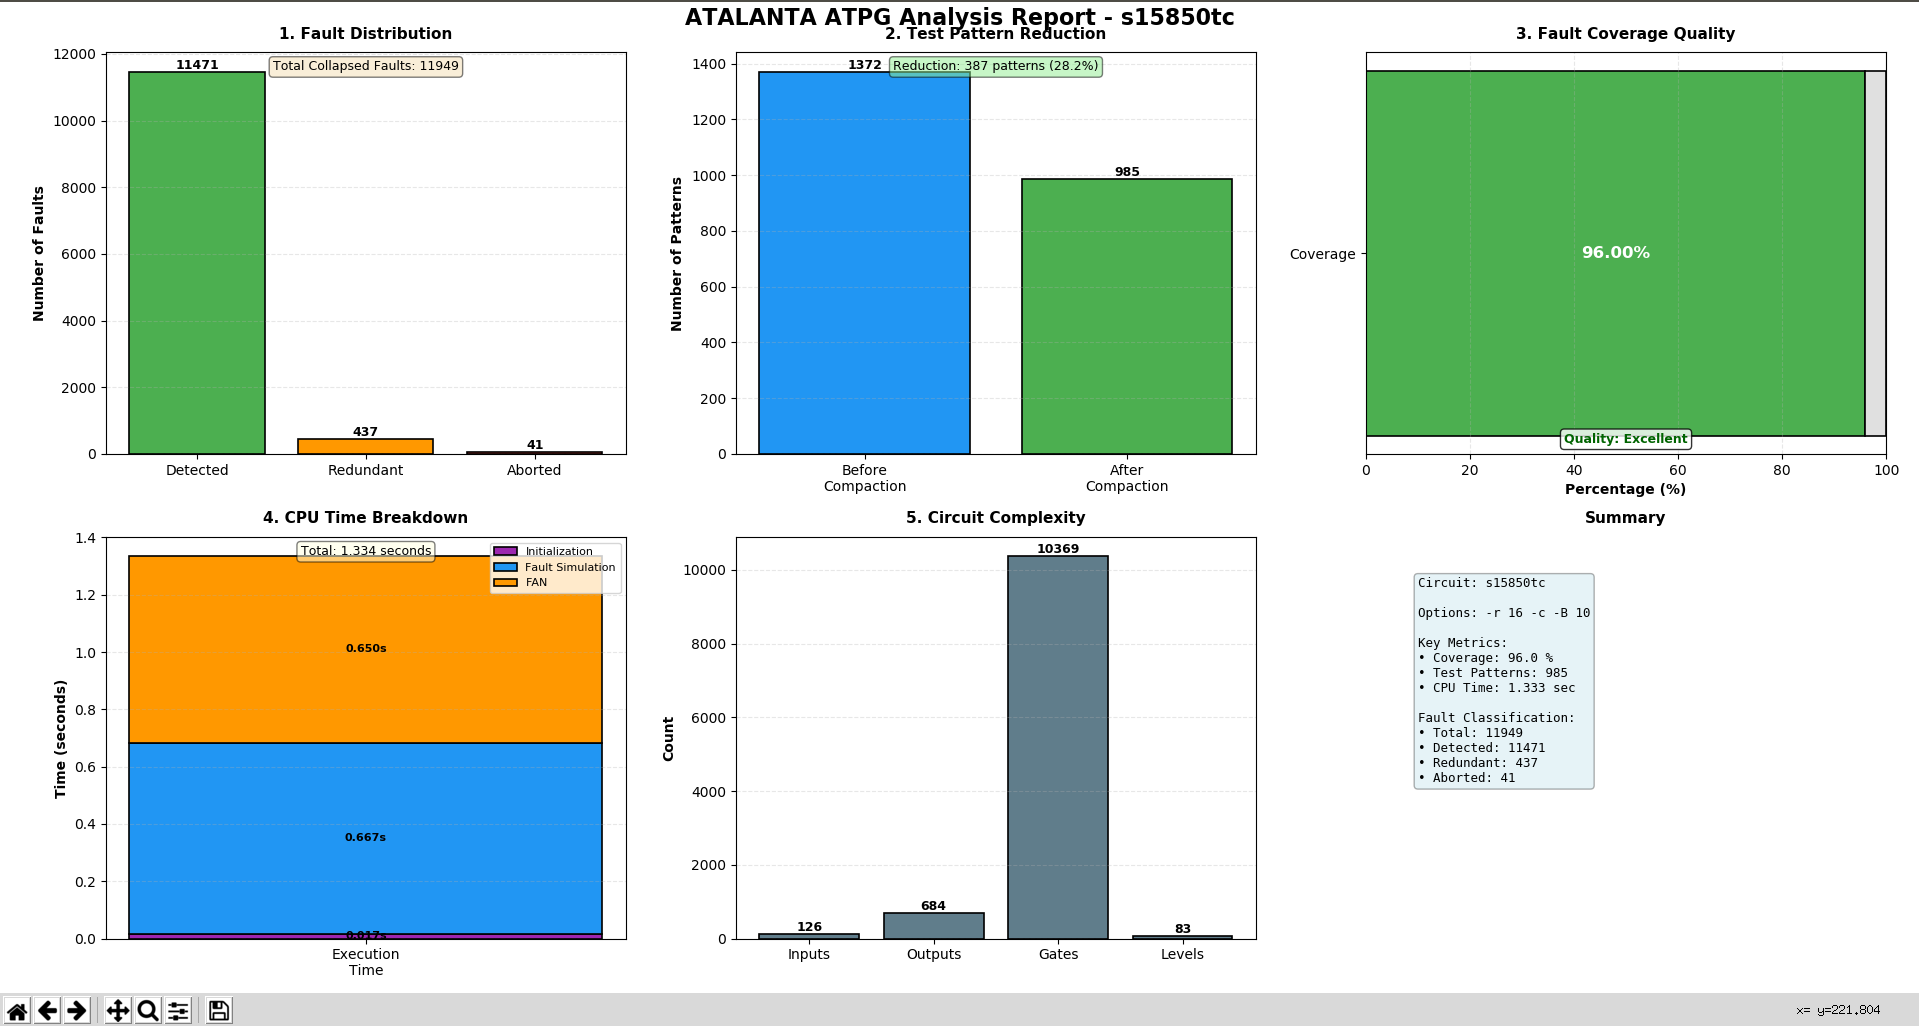
\includegraphics[width=0.48\textwidth]{images/s15850tc.png}
\caption{ATPG Analysis Results for s15850tc showing highest pattern compaction among sequential circuits}
\label{fig:s15850}
\end{figure}

\textbf{Results:} The s15850tc circuit achieved 96.0\% fault coverage as shown in Fig. \ref{fig:s15850}, detecting 11471 out of 11949 total faults in this deep sequential design. The circuit demonstrated the best pattern compaction among sequential benchmarks, reducing patterns from 1372 to 985, achieving an impressive 28.21\% reduction. Execution completed in 1.233 seconds with detailed breakdown of 0.017 seconds for initialization, 0.617 seconds for fault simulation, and 0.6 seconds for FAN algorithm. The ATPG process identified 437 redundant faults and encountered 41 aborted faults, with the high redundancy attributed to the circuit's deep sequential structure.

\subsubsection{s38417tc}
\textbf{Circuit Characteristics:} The s38417tc represents the largest sequential benchmark with 112 primary inputs, 1742 primary outputs, 23815 gates, and a circuit level of 48, combining large gate count with moderate sequential depth.

\textbf{ATPG Configuration:} Testing was conducted with compaction enabled (-c) and backtracking limit of 10 (-B 10).

\begin{figure}[h]
\centering
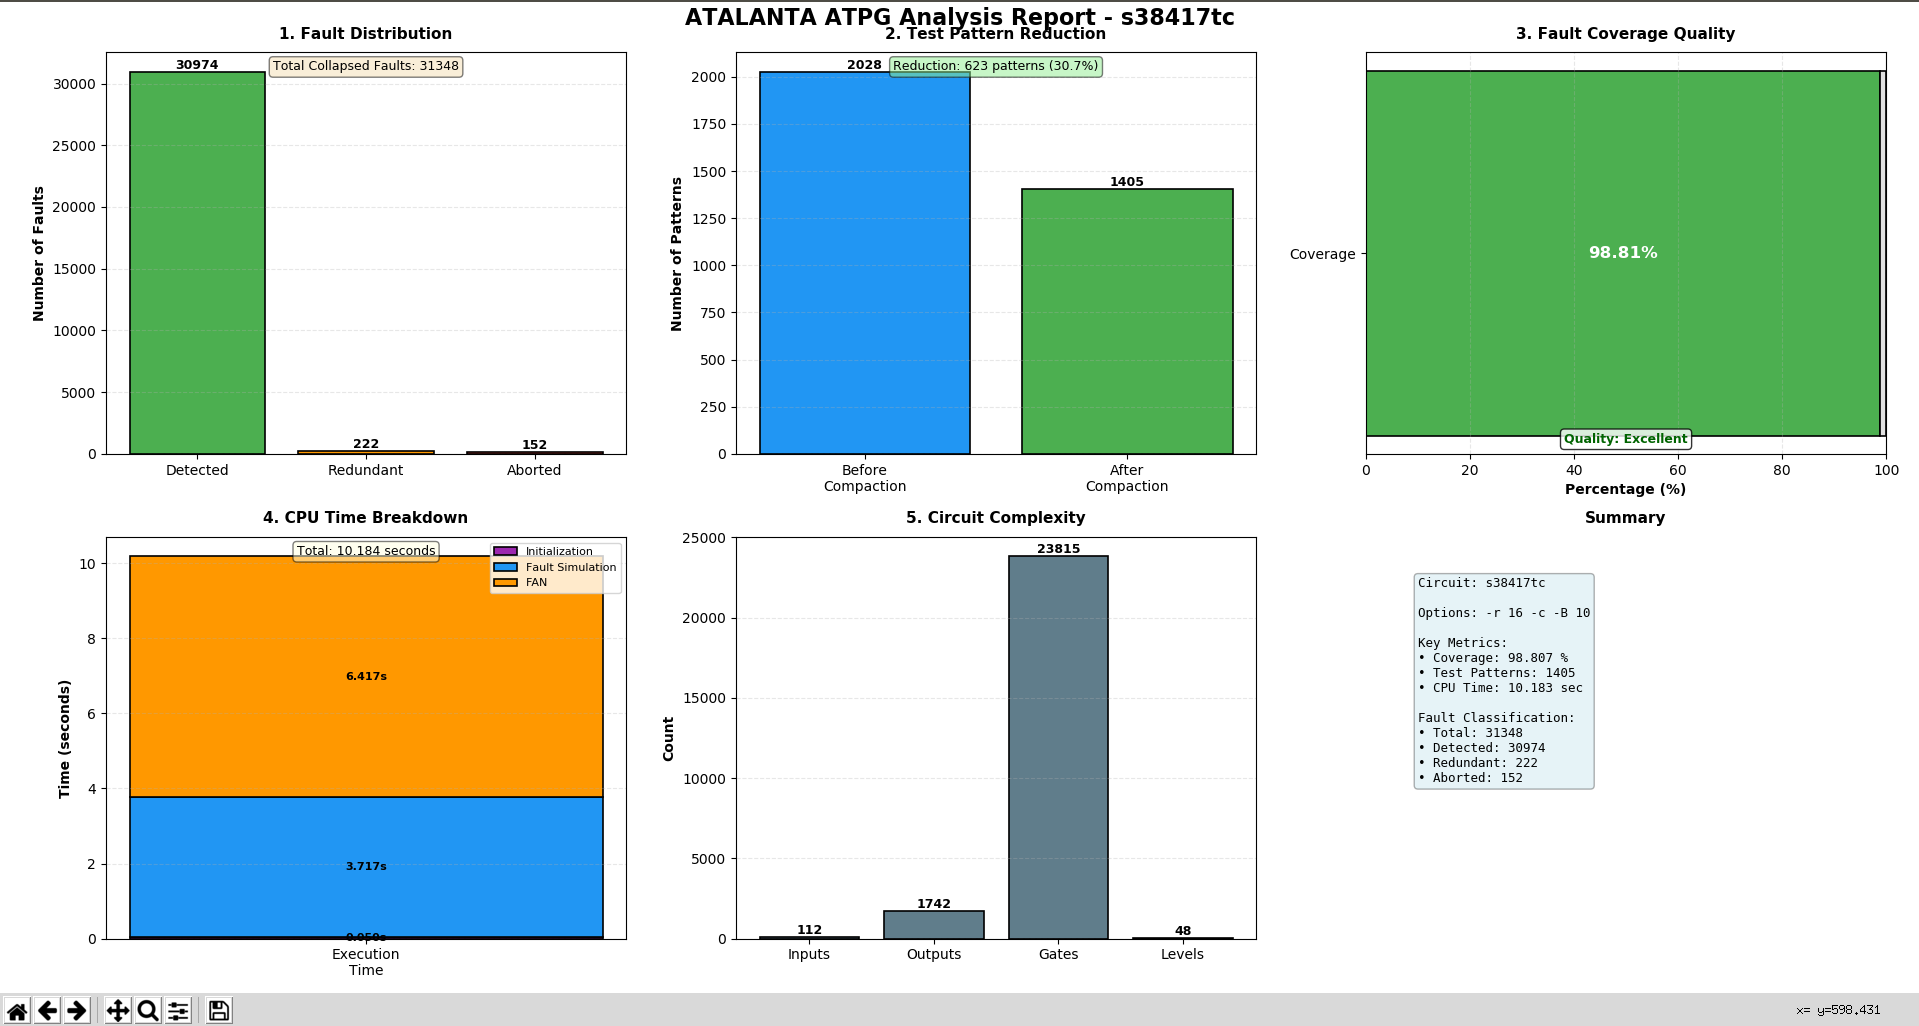
\includegraphics[width=0.48\textwidth]{images/s38417tc.png}
\caption{ATPG Analysis Results for s38417tc demonstrating best coverage and compaction among sequential circuits}
\label{fig:s38417}
\end{figure}

\textbf{Results:} The s38417tc circuit achieved the highest sequential coverage of 98.807\% as depicted in Fig. \ref{fig:s38417}, detecting 30974 out of 31348 total faults, approaching the performance of combinational circuits. The circuit demonstrated the best pattern compaction ratio, reducing patterns from 2028 to 1406, achieving an outstanding 30.67\% reduction, the highest among all tested circuits. Execution time was 9.017 seconds with distribution of 0.017 seconds for initialization, 3.017 seconds for fault simulation, and 5.983 seconds for FAN algorithm (the dominant phase). The ATPG identified 222 redundant faults and 152 aborted faults, with the higher abort count attributed to the large circuit size requiring more extensive test generation efforts.

\subsection{Batch Processing Analysis}

A batch execution was performed on 8 circuits (4 combinational + 4 sequential) to demonstrate the framework's capability for large-scale evaluation. Table \ref{tab:results} summarizes the key metrics for all circuits tested.

\begin{table}[htbp]
\caption{Experimental Results Summary for All Circuits}
\begin{center}
\begin{tabular}{|l|r|r|r|r|}
\hline
\textbf{Circuit} & \textbf{Gates} & \textbf{Coverage} & \textbf{Patterns} & \textbf{Time (s)} \\
\hline
\multicolumn{5}{|c|}{\textit{Combinational Circuits}} \\
\hline
half\_adder & 2 & 100.0\% & 4 & <0.001 \\
parity\_checker & 3 & 100.0\% & 5 & <0.001 \\
usbtc & 25871 & 99.316\% & 2875 & 19.367 \\
pcitc & 44433 & 99.826\% & 5945 & 92.167 \\
\hline
\multicolumn{5}{|c|}{\textit{Sequential Circuits}} \\
\hline
s9234tc & 5825 & 93.512\% & 775 & 0.567 \\
s13207tc & 8620 & 97.18\% & 1186 & 0.983 \\
s15850tc & 10369 & 96.0\% & 985 & 1.233 \\
s38417tc & 23815 & 98.807\% & 1406 & 9.017 \\
\hline
\multicolumn{5}{|c|}{\textit{Overall Statistics}} \\
\hline
\multicolumn{2}{|l|}{Average Coverage} & \multicolumn{3}{r|}{98.08\%} \\
\multicolumn{2}{|l|}{Average Time} & \multicolumn{3}{r|}{15.417 sec} \\
\multicolumn{2}{|l|}{Avg Pattern Reduction} & \multicolumn{3}{r|}{18.45\%} \\
\hline
\end{tabular}
\label{tab:results}
\end{center}
\end{table}

The batch processing results demonstrate comprehensive performance metrics across all eight circuits. The framework achieved an average fault coverage of 98.08\% with an average CPU time of 15.417 seconds per circuit, totaling 123.334 seconds for complete batch execution. Pattern compaction averaged 18.45\% reduction across all circuits, successfully processing 8 circuits and analyzing 185,907 total faults. The ATPG generated 18,649 patterns before compaction which were reduced to 15,176 patterns after compaction, demonstrating significant test time savings.

The results demonstrate that the framework successfully handles both simple 2-gate circuits and complex 44K-gate industrial controllers with consistent performance and comprehensive reporting. The two custom circuits (half\_adder and parity\_checker) achieved perfect 100\% fault coverage, while industrial controller benchmarks (usbtc and pcitc) demonstrated near-perfect coverage of 99.3-99.8\%. Sequential ISCAS benchmarks showed coverage ranging from 93.5\% (s9234tc) to 98.8\% (s38417tc), with the lower coverage attributed to higher complexity and sequential logic challenges.

\subsection{Configuration Trade-off Analysis}

Experiments were conducted with varying ATALANTA configurations to analyze trade-offs:

\textbf{Circuit Complexity vs. Execution Time:} The experimental results reveal clear correlation between circuit complexity and execution time. Simple circuits with fewer than 10 gates executed instantaneously in less than 0.001 seconds. Medium-complexity circuits ranging from 5000 to 10000 gates required 0.5 to 1.2 seconds for complete ATPG execution. Large industrial circuits with 20000 to 45000 gates demanded 9 to 92 seconds, with execution time scaling non-linearly with both gate count and circuit depth.

\textbf{Compaction Effectiveness:} Pattern reduction effectiveness varied significantly based on circuit complexity, ranging from 0\% for simple circuits with minimal patterns to 30.67\% for complex sequential circuits. The average reduction of 18.45\% across all circuits demonstrates substantial compaction effectiveness, with larger circuits consistently showing better compaction ratios. Simple combinational circuits with 2-3 gates achieved 0\% reduction as their patterns were already minimal. Complex combinational circuits ranging from 25000 to 45000 gates demonstrated 15.9\% to 29.3\% reduction. Sequential circuits with 5000 to 24000 gates achieved the best compaction ratios of 21.1\% to 30.7\%, indicating that sequential logic benefits most from pattern compaction algorithms.

\textbf{Fault Coverage Analysis:}
Combinational circuits achieved higher coverage (99.3-100\%) compared to sequential circuits (93.5-98.8\%), confirming the increased difficulty in testing sequential logic. Custom-designed simple circuits achieved perfect coverage, while large industrial controllers maintained near-perfect coverage despite their complexity.

\section{Conclusion}

This paper presented a comprehensive integrated framework for ATPG and fault simulation analysis with the primary objective of simplifying test generation workflows through user-friendly graphical interfaces and automated analysis capabilities. The framework successfully addresses the complexity barriers in ATPG evaluation by combining interactive execution, comprehensive metric extraction, professional visualization, and large-scale batch processing in a unified three-module architecture suitable for both educational instruction and research applications.

The framework's key contributions include an interactive GUI with real-time monitoring and configurable ATPG options, comprehensive result parsing that extracts over 25 circuit and test metrics, professional visualization suite with 5 distinct chart types for multi-dimensional result analysis, automated batch processing capability with CSV and formatted report generation, and robust support for both combinational and sequential circuit architectures. The implementation leverages Python Tkinter for cross-platform compatibility and Matplotlib for publication-quality visualization.

Experimental validation on eight benchmark circuits (4 combinational and 4 sequential) demonstrated exceptional performance with average fault coverage of 98.08\% and average pattern compaction of 18.45\%. Custom-designed simple circuits (half adder and parity checker) achieved perfect 100\% fault coverage with instant execution, while large industrial controller benchmarks (USB and PCI controllers with 25K-44K gates) maintained near-perfect coverage of 99.3-99.8\% despite their complexity. Sequential ISCAS benchmarks ranging from 5825 to 23815 gates achieved 93.5-98.8\% coverage with excellent compaction ratios of 21-31\%. The framework successfully analyzed 185,907 total faults across all circuits in 123.334 seconds cumulative execution time, generating 15,176 compacted patterns from an initial 18,649 patterns. The results confirm that execution time scales non-linearly with circuit complexity, ranging from sub-millisecond for simple circuits to 92 seconds for the largest 44K-gate benchmark.

Future enhancements may include multi-run comparison capabilities for statistical trend analysis across different ATPG configurations, integration with additional commercial and academic ATPG tools such as TetraMAX and HITEC for comparative studies, support for delay fault testing to address timing-related defects, machine learning-based ATPG parameter optimization to automatically tune configuration settings for maximum efficiency, and cloud-based batch processing infrastructure to handle large circuit libraries with distributed computing resources.

The framework source code and documentation are available for educational use, providing a valuable resource for Digital Fault Testing and Design for Testability courses.

\begin{thebibliography}{00}
\bibitem{b1} J. P. Roth, ``Diagnosis of automata failures: A calculus and a method,'' IBM Journal of Research and Development, vol. 10, no. 4, pp. 278-291, 1966.
\bibitem{b2} P. Goel, ``An implicit enumeration algorithm to generate tests for combinational logic circuits,'' IEEE Transactions on Computers, vol. C-30, no. 3, pp. 215-222, March 1981.
\bibitem{b3} H. Fujiwara and T. Shimono, ``On the acceleration of test generation algorithms,'' IEEE Transactions on Computers, vol. C-32, no. 12, pp. 1137-1144, Dec. 1983.
\bibitem{b4} I. Pomeranz and S. M. Reddy, ``On static compaction of test sequences for synchronous sequential circuits,'' in Proc. 33rd Design Automation Conference, 1996, pp. 215-220.
\bibitem{b5} M. L. Bushnell and V. D. Agrawal, Essentials of Electronic Testing for Digital, Memory and Mixed-Signal VLSI Circuits. Springer, 2000.
\bibitem{b6} H. K. Lee and D. S. Ha, ``ATALANTA: An efficient ATPG for combinational circuits,'' Technical Report 93-12, Dept. of Electrical Eng., Virginia Polytechnic Institute and State University, 1993.
\bibitem{b7} M. Abramovici, M. A. Breuer, and A. D. Friedman, Digital Systems Testing and Testable Design. IEEE Press, 1990.
\bibitem{b8} F. Brglez, D. Bryan, and K. Kozminski, ``Combinational profiles of sequential benchmark circuits,'' in Proc. IEEE International Symposium on Circuits and Systems, 1989, pp. 1929-1934.
\bibitem{b9} V. D. Agrawal, K. T. Cheng, and P. Agrawal, ``CONTEST: A concurrent test generator,'' in Proc. 25th ACM/IEEE Design Automation Conference, 1988, pp. 84-89.
\bibitem{b10} T. Niermann and J. H. Patel, ``HITEC: A test generation package for sequential circuits,'' in Proc. European Design Automation Conference, 1991, pp. 214-218.
\bibitem{b11} M. S. Hsiao, E. M. Rudnick, and J. H. Patel, ``Sequential circuit test generation using dynamic state traversal,'' in Proc. European Design and Test Conference, 1997, pp. 22-28.
\bibitem{b12} W. T. Cheng and T. J. Chakraborty, ``GENTEST: An automatic test-generation system for sequential circuits,'' IEEE Computer, vol. 22, no. 2, pp. 43-49, Feb. 1989.
\end{thebibliography}

\end{document}
